%% Nube de los 312 escenarios admisibles. Generada desde
%% code/caballero/caballero_caso_chileno_resultados.csv.
\begin{figure}[H]
\centering
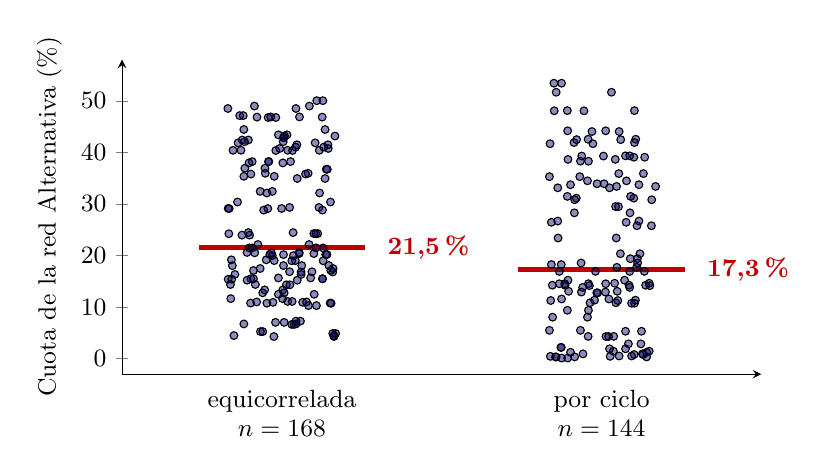
\begin{tikzpicture}
\begin{axis}[
    width=0.80\textwidth, height=0.46\textwidth,
    xmin=0.5, xmax=2.5, ymin=-3, ymax=58,
    xtick={1,2},
    xticklabels={{\shortstack{equicorrelada\\$n=168$}},{\shortstack{por ciclo\\$n=144$}}},
    ylabel={Cuota de la red Alternativa (\%)},
    ytick={0,10,20,30,40,50},
    axis lines=left, axis x line*=bottom, xtick style={draw=none},
    tick label style={font=\small}, label style={font=\small}, clip=false]
\addplot[only marks, mark=*, mark size=1.4pt, draw=none,
         fill=blue!45!black, fill opacity=0.45] coordinates {(1.043,41.02) (1.135,34.94) (1.094,16.86) (0.907,38.21) (0.932,32.44) (1.127,15.50) (0.832,15.41) (1.109,50.02) (1.101,12.49) (0.989,43.40) (0.933,5.26) (0.925,22.14) (0.917,14.39) (0.981,46.76) (1.002,11.65) (1.018,40.41) (1.168,4.89) (1.100,20.38) (1.042,19.02) (1.166,43.17) (0.903,15.51) (0.884,36.93) (1.038,6.65) (0.845,18.05) (0.842,19.17) (1.005,42.85) (0.989,15.66) (1.142,36.73) (1.044,6.74) (1.005,18.06) (0.999,29.13) (0.914,48.98) (0.834,24.23) (0.895,42.40) (1.065,10.93) (0.898,21.49) (0.956,29.11) (0.831,48.51) (1.112,24.26) (0.883,42.07) (0.921,11.00) (1.129,21.47) (1.003,37.96) (1.118,32.13) (1.048,15.22) (1.082,35.95) (0.861,30.38) (1.014,14.33) (1.003,13.34) (1.126,46.84) (0.953,10.76) (1.033,40.37) (0.850,4.49) (0.962,20.19) (0.940,12.77) (0.881,44.44) (1.108,10.30) (0.959,38.22) (1.163,4.30) (1.031,18.99) (1.036,19.99) (1.047,41.48) (1.060,16.34) (0.881,35.36) (0.980,7.04) (0.911,17.10) (0.967,20.53) (0.863,41.85) (1.159,16.81) (0.903,35.80) (1.058,7.28) (0.932,17.49) (1.127,28.81) (1.055,46.87) (0.875,23.96) (1.117,40.40) (1.151,10.79) (1.137,20.20) (1.024,29.33) (0.879,47.13) (0.895,24.46) (1.145,40.76) (1.018,11.10) (0.891,20.60) (1.131,41.02) (1.048,34.94) (1.024,16.86) (0.958,38.21) (0.970,32.44) (0.911,15.50) (0.843,15.41) (1.128,50.02) (0.989,12.49) (1.016,43.40) (0.940,5.26) (1.085,22.14) (0.839,14.39) (0.957,46.76) (0.840,11.65) (0.872,40.41) (1.159,4.89) (1.054,20.38) (0.976,19.02) (1.008,43.17) (1.127,15.51) (0.947,36.93) (1.031,6.65) (1.062,18.05) (0.951,19.17) (1.006,42.85) (1.090,15.66) (1.139,36.73) (0.881,6.74) (1.147,18.06) (0.832,29.13) (1.086,48.98) (1.106,24.23) (0.876,42.40) (0.972,10.93) (1.107,21.49) (0.835,29.11) (1.044,48.51) (1.100,24.26) (1.004,42.07) (1.077,11.00) (0.907,21.47) (0.897,37.96) (0.953,32.13) (0.891,15.22) (0.948,35.95) (1.152,30.38) (1.025,14.33) (0.946,13.34) (0.922,46.84) (1.154,10.76) (0.981,40.37) (1.163,4.49) (1.005,20.19) (1.007,12.77) (1.135,44.43) (1.083,10.30) (1.027,38.22) (0.975,4.30) (1.129,18.99) (0.970,19.99) (1.144,41.48) (0.853,16.34) (0.976,35.36) (1.007,7.04) (1.153,17.10) (0.915,20.53) (1.104,41.85) (1.060,16.81) (1.074,35.80) (1.044,7.28) (1.160,17.49) (0.943,28.81) (0.965,46.87) (0.899,23.96) (0.847,40.40) (0.902,10.79) (1.141,20.20) (1.116,29.33) (0.868,47.13) (1.035,24.45) (0.993,40.76) (1.032,11.10) (1.054,20.60) };
\addplot[only marks, mark=*, mark size=1.4pt, draw=none,
         fill=blue!45!black, fill opacity=0.45] coordinates {(1.934,38.30) (2.157,30.82) (1.988,12.77) (2.044,29.49) (2.046,23.40) (1.893,9.39) (1.851,53.41) (1.970,44.04) (2.090,19.39) (2.107,42.55) (2.078,34.48) (1.868,14.53) (2.141,1.24) (2.103,41.90) (2.128,0.94) (2.008,33.92) (2.141,0.34) (1.846,14.25) (1.840,0.46) (1.837,35.30) (1.916,0.35) (1.915,28.28) (1.894,0.13) (2.023,11.58) (1.843,18.26) (2.031,51.66) (1.886,14.24) (2.060,42.47) (1.837,5.50) (1.936,18.56) (2.149,14.63) (2.013,44.18) (2.106,11.35) (2.054,35.89) (2.038,4.33) (1.895,15.22) (2.025,33.13) (1.843,26.45) (2.103,10.75) (2.156,25.78) (2.120,20.35) (1.847,8.05) (1.945,48.06) (1.938,39.29) (1.868,16.92) (2.043,38.65) (2.101,31.13) (1.937,12.92) (2.123,2.88) (2.101,39.06) (1.874,2.20) (2.091,31.47) (2.130,0.81) (1.897,13.07) (2.025,1.92) (2.047,33.40) (2.037,1.46) (1.863,26.69) (2.055,0.53) (2.045,10.85) (2.110,17.72) (2.103,48.10) (1.941,13.82) (2.075,39.33) (2.125,5.32) (2.134,16.94) (1.885,14.54) (1.839,41.68) (2.051,11.28) (1.903,33.73) (2.022,4.30) (2.151,14.16) (1.959,38.29) (1.916,30.82) (1.985,12.77) (2.053,29.48) (1.864,23.40) (1.959,9.39) (1.875,53.41) (2.055,44.04) (2.112,19.39) (1.958,42.55) (1.956,34.49) (2.013,14.53) (1.903,1.24) (1.914,41.90) (1.942,0.94) (1.986,33.92) (1.858,0.34) (2.086,14.25) (2.027,0.46) (1.932,35.30) (1.856,0.35) (2.089,28.28) (1.875,0.13) (1.875,11.58) (1.874,18.26) (1.858,51.66) (2.138,14.24) (1.922,42.47) (1.934,5.50) (2.113,18.56) (2.041,14.63) (1.894,44.18) (1.978,11.35) (2.131,35.89) (1.958,4.33) (2.072,15.22) (1.863,33.13) (2.077,26.45) (2.094,10.75) (2.111,25.78) (2.059,20.35) (1.956,8.05) (1.852,48.06) (2.006,39.29) (2.088,16.92) (1.895,38.64) (1.921,31.13) (2.012,12.92) (2.084,2.88) (2.135,39.06) (1.873,2.20) (1.893,31.47) (2.102,0.81) (2.049,13.07) (2.075,1.92) (2.169,33.40) (2.149,1.46) (2.117,26.69) (2.094,0.53) (1.964,10.85) (2.048,17.72) (1.893,48.10) (2.088,13.82) (2.088,39.33) (2.075,5.32) (1.981,16.94) (1.959,14.54) (1.973,41.68) (1.841,11.28) (2.117,33.73) (2.014,4.30) (1.962,14.17) };
\addplot[red!75!black, line width=1.8pt] coordinates {(0.74,21.48) (1.26,21.48)};
\addplot[red!75!black, line width=1.8pt] coordinates {(1.74,17.31) (2.26,17.31)};
\node[red!75!black, font=\small\bfseries, anchor=west] at (axis cs:1.30,21.48) {21,5\,\%};
\node[red!75!black, font=\small\bfseries, anchor=west] at (axis cs:2.30,17.31) {17,3\,\%};
\end{axis}
\end{tikzpicture}
\caption[Cuota de la red Alternativa sobre los escenarios admisibles]{Cuota de
la actividad que el modelo asigna a la red Alternativa, con un punto por cada
uno de los 312 escenarios admisibles y la mediana de cada grupo en rojo. La
dispersión vertical es el desplazamiento horizontal aleatorio que separa puntos
de igual valor. Elaboración propia.}
\label{fig:escenarios-admisibles}
\end{figure}
